% PLANTILLA PARA TRABAJOS EN LATEX
% Autor: Manuel Gachs Ballegeer
% Github: https://github.com/Manuelbelgicano
% Licencia: GNU General Public License v3.0
% Versión: 0.1

\documentclass[11pt,twoside,titlepage,a4paper]{article}

%%%%%%%%%%%%%%%%%%%%%%%%%%%%%%%%%%%%%%%%%
%			   COLORINES				%
%%%%%%%%%%%%%%%%%%%%%%%%%%%%%%%%%%%%%%%%%
\usepackage{xcolor}
\definecolor{rojooscuro}{HTML}{8A0808}
\definecolor{burdeos}{HTML}{610B0B}
\definecolor{rojomorado}{HTML}{B40431}

%%%%%%%%%%%%%%%%%%%%%%%%%%%%%%%%%%%%%%%%%
%			  MATEMÁTICAS				%
%%%%%%%%%%%%%%%%%%%%%%%%%%%%%%%%%%%%%%%%%
\usepackage{amsmath} % Matemáticas
\usepackage{amsfonts} % Letras caligráficas para matemáticas
\usepackage{mathtools} % Matemáticas extra
\usepackage{amsthm} % Teoremas
% Eliminar '*' para añadir numeración a los lemas, teoremas...
\theoremstyle{definition}
\newtheorem*{defi}{Definición} % Comando para las definiciones
\newtheoremstyle{plain_rojo}{}{}{}{}{\color{rojooscuro}\bfseries}{:}{ }{}
\theoremstyle{plain_rojo}
\newtheorem*{lem}{Lema} % Comando para los lemas
\newtheorem*{teo}{Teorema} % Comando para los teoremas
\theoremstyle{remark}
\newtheorem*{cor}{Corolario} % Comando para los corolarios
\renewenvironment{proof}{{\bfseries\color{rojooscuro}Demostración:}}{\qed} % Cambiar el título de las demostraciones

%%%%%%%%%%%%%%%%%%%%%%%%%%%%%%%%%%%%%%%%%
%			   TIPOGRAFÍA				%
%%%%%%%%%%%%%%%%%%%%%%%%%%%%%%%%%%%%%%%%%
\usepackage[sfdefault]{roboto}  %% Option 'sfdefault' only if the base font of the document is to be sans serif
\usepackage[T1]{fontenc}

%%%%%%%%%%%%%%%%%%%%%%%%%%%%%%%%%%%%%%%%%
%				  CÓDIGO				%
%%%%%%%%%%%%%%%%%%%%%%%%%%%%%%%%%%%%%%%%%
\usepackage{listingsutf8}
\lstset{
	inputencoding=utf8/latin1, % Codificación
	xleftmargin=1em, % Margen extra a la izquierda
	breaklines=true, % Romper líneas largas
	language=C++, % Lenguaje del código
	frame=single, % Enmarcado
	numbersep=8pt, % Separación de los números de línea
	tabsize=4, % Tamaño de los tabs
	frame=leftline, % Posición del enmarcado
	framerule=2pt, % Grosor del enmarcado
	showstringspaces=false, % Mostrar los espacios en las cadenas de caracteres
	basicstyle=\ttfamily, % Estilo del código
	keywordstyle=\color{burdeos}, % Estilo de las palabras reservadas
	numberstyle=\normalfont, % Estilo de los números de línea
	rulecolor=\color{rojooscuro}, % Estilo del enmarcado
	commentstyle=\color{red}, % Estilo de los comentarios
	stringstyle=\color{rojomorado} % Estilo de las cadenas de caracteres
}

%%%%%%%%%%%%%%%%%%%%%%%%%%%%%%%%%%%%%%%%%
%				MÁRGENES				%
%%%%%%%%%%%%%%%%%%%%%%%%%%%%%%%%%%%%%%%%%
\usepackage[a4paper]{geometry}
\geometry{
	left=3cm, % Margen izquierdo
	right=3cm, % Margen derecho
	bottom=3cm % Margen inferior
}

%%%%%%%%%%%%%%%%%%%%%%%%%%%%%%%%%%%%%%%%%
%  			  LISTAS/TABLAS				%
%%%%%%%%%%%%%%%%%%%%%%%%%%%%%%%%%%%%%%%%%
\usepackage{multirow} % Cosas chulas para las tablas
\usepackage{enumitem} % Opciones de personalización de listas
\renewcommand{\arraystretch}{1.3} %Cambiar el tamaño entre líneas de una tabla

%%%%%%%%%%%%%%%%%%%%%%%%%%%%%%%%%%%%%%%%%
%		COMANDOS PERSONALIZADOS 		%
%%%%%%%%%%%%%%%%%%%%%%%%%%%%%%%%%%%%%%%%%
\newcommand{\autores}{ % Autores del documento
	\begin{tabular}{l}
	Jesús Miguel Rojas Gómez \\
	Javier Ojeda Baena \\
	Ignacio Garach Vélez \\
	Guillermo Ramblado Carrasco \\
	Manuel Gachs Ballegeer	
	\end{tabular}
}
\newcommand{\institucion}{ % Insitución
	Sistemas Operativos
}
\newcommand{\infoextra}{ % Año o cualquier otra información para el título
	Universidad de Granada
}

%%%%%%%%%%%%%%%%%%%%%%%%%%%%%%%%%%%%%%%%%
%		ENCABEZADO/PIE DE PAGINA		%
%%%%%%%%%%%%%%%%%%%%%%%%%%%%%%%%%%%%%%%%%
\usepackage{fancyhdr}
\setlength{\headheight}{14pt}
\pagestyle{fancy}
\fancyhf{}
% Para que aparezca el título de la sección y no el número 
\renewcommand{\sectionmark}[1]{%
\markboth{#1}{}}
% Encabezado
\fancyhead[LE,RO]{\color{burdeos}{\leftmark}} % A la izquierda en pares, derecha en impares
\fancyhead[RE,LO]{\color{burdeos}{\institucion}} % A la derecha en pares, izquierda en impares
% Pie de página
\fancyfoot[LE,RO]{\Large\textbf{\thepage}} % A la izquierda en pares, derecha en impares
\renewcommand{\headrulewidth}{0.5pt} % Grosor de la línea

%%%%%%%%%%%%%%%%%%%%%%%%%%%%%%%%%%%%%%%%%
%			   	TÍTULOS					%
%%%%%%%%%%%%%%%%%%%%%%%%%%%%%%%%%%%%%%%%%
\usepackage{titlesec}
\titleformat{\section} % Estilo de las secciones
{\color{rojooscuro}\fontsize{13}{15}\bfseries}
{\color{rojooscuro}\thesection}{1em}{}

%%%%%%%%%%%%%%%%%%%%%%%%%%%%%%%%%%%%%%%%%
%		   	  MISCELÁNEO				%
%%%%%%%%%%%%%%%%%%%%%%%%%%%%%%%%%%%%%%%%%
\usepackage{pagecolor} % Colorear las portadas
\renewcommand{\contentsname}{Índice} % Cambiar el título del índice
\setlength\parindent{0pt} % Tamaño de la sangría
\usepackage{graphicx} % Imágenes
\renewcommand{\figurename}{Figura} % Cambiar el título de las etiquetas de las figuras
\usepackage{hyperref} % Las referencias
\usepackage{url}

\usepackage{graphicx}
\begin{document}

%%%%%%%%%%%%%%%%%%%%%%%%%%%%%%%%%%%%%%%%%
%				 PORTADA 				%
%%%%%%%%%%%%%%%%%%%%%%%%%%%%%%%%%%%%%%%%%
\begin{titlepage}
	\newpagecolor{rojooscuro} % Color de la portada
	\parbox[t]{\textwidth}{
		\raggedright
		\color{white}{\LARGE{\textbf{\institucion}}} \\
		\textit{\infoextra}
	}
	\vfill
	\parbox[c]{\textwidth}{
		\color{white}{
			\fontsize{70pt}{70pt}{\textbf{UML}} \\
			\bigskip \\
			\fontsize{40pt}{40pt}{\emph{Linux User Mode Linux}}
		}
	}
	\vfill
	\parbox[t]{\textwidth}{
		\raggedright
		\color{white}{\Large{\autores}} \\
		\raggedleft
		\color{white}{\emph{noviembre 2019}}
	}
\end{titlepage}
\restorepagecolor

%%%%%%%%%%%%%%%%%%%%%%%%%%%%%%%%%%%%%%%%%
%				 ÍNDICE 				%
%%%%%%%%%%%%%%%%%%%%%%%%%%%%%%%%%%%%%%%%%
\tableofcontents
\clearpage

%%%%%%%%%%%%%%%%%%%%%%%%%%%%%%%%%%%%%%%%%
%				 DOCUMENTO 				%
%%%%%%%%%%%%%%%%%%%%%%%%%%%%%%%%%%%%%%%%%

\section{Introducción}

En muchas ocasiones, puede resultar ventajoso o interesante dividir los
recursos de una máquina en varios entornos de ejecución. La 
\textbf{virtualización} es la herramienta que se utiliza en la informática
para poder aprovecharlo. Sin embargo, la virtualización es solamente una
abstracción. En la práctica, son piezas de software las que realizan esta 
función. En este documento abarcaremos únicamente una de las diversas formas 
de obtener virtualización: \textbf{UML}, siglas para \textit{user-mode linux}.
La razón de esta elección es conocer y entender la herramienta que ya hemos 
utilizado en el módulo práctico de administración de sistemas de la 
asignatura, y a la que no hemos prestado atención.
\\

Primero definiremos qué es exactamente \textbf{UML}, seguido por sus 
principales características. Tras eso explicaremos brevemente cómo instalarlo 
y cuál es su funcionamiento. Después, expondremos algunas de sus principales
aplicaciones, con especial hincapié en el campo de la ciberseguridad y de los
servidores. Finalmente terminaremos con algunas conclusiones acerca de la
herramienta.

\section{¿Qué es UML?}

A la hora de plantearse el hecho de querer montar una máquina virtual, 
tenemos a nuestra disposición múltiples opciones. Algunas de ellas son 
comerciales tales como VMWARE o Virtual PC, que soportan  una amplia variedad 
de sistemas, además de poseer sólidas interfaces gráficas, aunque cada una de 
ellas incluyen sus respectivos costos. De igual forma, podemos encontrar 
versiones libres como coLinux o \textbf{UML} (\textit{user mode linux}), 
la cual nos ofrece un gran rendimiento con bastante simplicidad, además de no 
requerir ningún programa adicional de virtualización.
\\

\textbf{UML} es una aplicación que solamente se puede ejecutar sobre sistemas 
GNU/LINUX, proporcionándonos un sistema operativo Linux virtual. Más 
detalladamente, consiste en crear una adaptación a la interfaz software 
definida por el núcleo en lugar de generar esa adaptación a la interfaz 
hardware. El objetivo de todo este proceso es transformar el núcleo con el 
fin de que pueda ser ejecutado sobre un sistema físico en una aplicación de 
nivel de usuario en la que todos los dispositivos son virtuales. Es decir, se 
realiza la ejecución de varios núcleos Linux, con sus propios espacios de 
usuario asignados, en el contexto de un sólo núcleo Linux.
\\

En resumen, todo lo que se realiza es parchear el núcleo de Linux de SO 
invitado con el parche de \textbf{UML}, consiguiendo ejecutar este nuevo 
núcleo en el sistema anfitrión como un sistema operativo separado, tal que 
tras ejecutar el núcleo parcheado con \textbf{UML}, todo lo que se necesita 
es aportar un sistema de archivos para poder usar, obteniendo finalmente un 
sistema Linux independiente ejecutado en tu computadora. Así, el nuevo núcleo 
que se consigue tras el parche supone una aplicación en espacio de usuario 
que se va a estar ejecutando sobre el núcleo real (SO anfitrión).
\\

El principal objetivo de \textbf{UML} fue, desde un principio, lograr 
desarrollar el kernel del sistema operativo de una forma más fácil para 
evitar reiniciar el sistema ante la aparición de cualquier problema. Gracias 
a \textbf{UML}, esto no es necesario, ya que únicamente bastaría con matar el 
proceso y volver un paso atrás.
\\

Inicialmente se desarrolló para la arquitectura x86, aunque hoy en día está 
disponible en otras como ia64 y PowerPC. 
\\

\textbf{UML} se encuentra implementado en el núcleo de Linux desde la versión 
del kernel 2.6, pero debe ser activado y recompilado antes de poder 
utilizarse. Tal y como está descrito, se encarga de virtualizar dispositivos 
y permite a los sistemas operativos alojados la compartición de todos esos 
dispositivos existentes, ya sean unidades CD-ROM, sistemas de ficheros, etc.

\begin{figure}[htp]
\centering
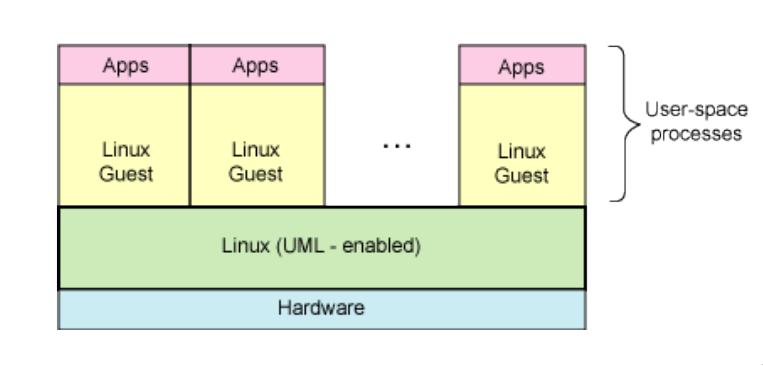
\includegraphics[scale=0.50]{figura_1.png}
\caption{Esquema de funcionamiento de UML}
\label{}
\end{figure}

\section{Principales características}

A grandes rasgos podemos decir que \textbf{UML} es una aplicación que sólo se 
puede ejecutar sobre sistemas GNU/Linux y que nos proporciona un sistema 
operativo Linux virtual.
\\

\begin{figure}[htp]
\centering
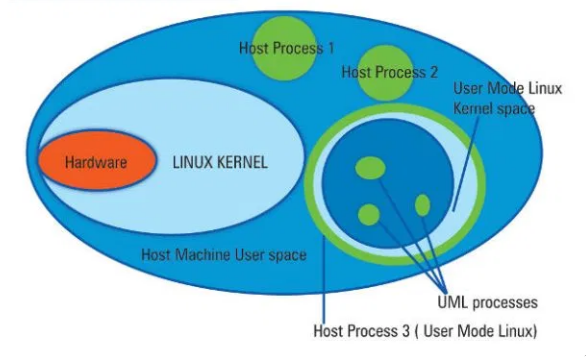
\includegraphics[scale=0.50]{figura_2.png}
\caption{Composición de UML}
\label{}
\end{figure}

Más específicamente el \textbf{UML} es una adaptación del núcleo de Linux 
como las que se hacen para ejecutarlo en diferentes procesadores, con la 
diferencia que en este caso es una adaptación a la interfaz software definida 
por el núcleo y no a la interfaz hardware definida por los componentes 
físicos. Esto se muestra claramente en la figura anteriormente incluída.
\\

En realidad \textbf{UML} lo que hace es transformar un núcleo pensado para un 
sistema físico en una aplicación a nivel de usuario en la que todos los 
dispositivos son virtuales, con todo lo que ello conlleva, sus ventajas e 
inconvenientes:

\begin{itemize}[font={\color{rojooscuro}\bfseries}]
\item Una de las grandes ventajas es la facilidad de uso y montaje de un 
sistema de archivos en el mismo. Es muy intuitivo a la hora de realizar las 
configuraciones pertinentes, al fin y al cabo, no es mas que “otro Linux 
dentro de Linux”.
\item Un sistema de virtualización con \textbf{UML} es más lento que un 
sistema de virtualización a nivel del sistema operativo, ya que estamos 
ejecutando el núcleo como proceso, pero por otro lado tenemos la ventaja de 
que estamos seguros de que la máquina virtual está claramente aislada del 
sistema real y de otras máquinas virtuales como ella, lo cual nos da mucha 
protección respecto alas consecuencias de los problemas generados por el 
código que se ejecuta dentro de cada máquina virtual.
\item En el caso que \textbf{UML} se cuelgue, el kernel principal del sistema 
anfitrión no se verá afectado.
\item No se producen daños en los componentes físicos por tratarse de una 
“simulación”.
\item Utilización de modo root sin riesgo de dañar configuraciones y 
corromper archivos del sistema anfitrión.
\item \textbf{UML} puede correrse como un usuario cualquiera, lo cual es 
sumamente recomendable, ya que se evitan posibles modificaciones que se 
puedan realizar si montamos sistemas de ficheros de la máquina host en la 
maquina virtual.
\item Se pueden realizar procesos de depuración, perfilar aplicaciones de 
usuario, entre otros como si fueran procesos normales (con la ventaja de que 
si hay cuelgues nuestro sistema sigue funcionando).
\item Se pueden probar nuevas versiones de kernel, quizá hasta tratar de 
desarrollar módulos para el kernel. Además se puede probar diferentes 
distribuciones de linux, algo muy útil cuando se está dilucidando la elección 
de una u otra.
\item Tiene un rendimiento más bajo que algunas tecnologías de la
competencia, como Xen y OpenVZ. El trabajo futuro para agregar soporte para la virtualización x86 a \textbf{UML} puede reducir esta desventaja.
\end{itemize}

A menudo citado como una fortaleza de Xen (una tecnología competitiva) es el 
soporte para el almacenamiento local de subprocesos. Esto ahora también es 
compatible con los últimos núcleos \textbf{UML}. Xen se concentra en 
virtualizar toda la máquina y, por lo tanto, todos los sistemas que se 
ejecutan en una máquina Xen son realmente máquinas virtuales. En
\textbf{UML}, la máquina \emph{host} no está virtualizada de ninguna manera,
y solo los sistemas invitados son verdaderas máquinas virtuales. Esto permite 
el acceso directo de invitados UML a los sistemas de archivos y hardware del 
\emph{host}, donde es común asignar un directorio de \emph{host} (por 
ejemplo, /uml/root$\rightarrow$/).
\\

Como desventajas de \textit{user-mode linux}, podemos listar las siguientes:
\begin{itemize}[font={\color{rojooscuro}\bfseries}]
\item Como se ha señalado anteriormente, es más lento que otros sistemas de
virtualización.
\item Para acceder a los componentes hardware de la máquina desde \textbf{UML}
es necesario instalar controladores de \textit{user-mode linux} adicionales.
\item No se puede utilizar para depurar código de kernel que sea dependiente
de la arquitectura del sistema.
\item Solamente puede ser utilizado en sistemas Linux.
\end{itemize}

\begin{figure}[htp]
\centering
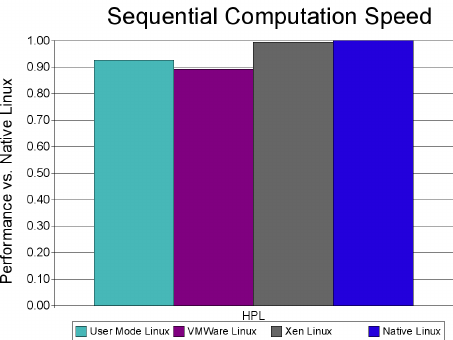
\includegraphics[scale=0.80]{figura_5.png}
\caption{Comparación de velocidad computacional en diferentes herramientas de virtualización}
\label{}
\end{figure}

\section{Instalación y funcionamiento}

\textbf{UML} permite a los desarrolladores de kernel implementar nuevas 
funciones y tocar ciertos archivos fundamentales para el sistema sin que 
estos sufran daño, evitando que provoquen un fallo irreparable en el sistema 
y no se pueda arrancar (uno de los archivos es \texttt{sys-libs/glibc} donde 
hay librerías y muchas funciones muy importantes para el sistema).

\subsection*{\color{burdeos}{Instalación}}

Para la instalación necesitamos descargarnos un árbol de kernel y extraerlo 
en alguna ubicación de desarrollo local, por ejemplo, en el directorio de 
inicio del usuario actual. Una vez descomprimido, pasaríamos a configurar el 
kernel. Para ello pondremos los siguientes comandos en el directorio donde 
hayamos extraído el núcleo:
\begin{lstlisting}
~$ cd <nombre del kernel descargado>
~$ ARCH= um menuconfig
\end{lstlisting}
Algunas configuraciones recomendadas para que el kernel sea completamente 
funcional se pueden encontrar en este \href{https://web2.clarkson.edu/class/cs644/kernel/setup/uml/uml.html}{enlace}.
En este momento podemos construir el kernel de Linux:
\begin{lstlisting}
~$ ARCH= um linux
\end{lstlisting}
Por último, deberemos crear un sistema de archivos. Para ello, los pasos a 
seguir son los siguientes:
\begin{enumerate}[font={\color{rojooscuro}\bfseries}]
\item Realizamos una partición y luego inicializamos mediante la
función fdisk.
\item Creamos la raíz de montaje.
\item Instalamos el sistema de archivos.
\end{enumerate}
En la página web a la que nos hemos referido anteriormente, se utiliza Debian 
para realizar la creación del sistema de archivos, ya que su instalación en 
el \textbf{UML} es sencilla.
\\

La cantidad de memoria que posee un \textbf{UML} es controlada por el campo \texttt{mem=}. Por ejemplo, \texttt{mem=128M} otorgará al \textbf{UML} 128 megabytes de memoria "física". El tamaño es especificado como un número seguido de 'k', 'K', 'm', 'M', 'g' o 'G', que posee el siguiente significado: kilobits, kilobytes, megabits, megabytes, gigabits y gigabytes respectivamente. El mayor tamaño de memoria "física" posible en arquitectura x86 es 3G, y en x86\_64 es 266G.
\\

\textbf{UML} tiene consolas y líneas seriales, que son prácticamente idénticas. Se pueden conectar a una variedad de dispositivos host diferentes, incluidos descriptores de archivos ya abiertos, pseudo terminales y puertos.
Estos son los más comunes:
\begin{center}
\begin{tabular}{|c|p{11.4cm}|}
\hline
\parbox[t]{3cm}{\texttt{con0=fd:0,fd:1} \texttt{con=pts}}
& La consola principal está conectada está conectada con \texttt{stdin} y
\texttt{stdout}, y el resto de consolas están conectadas a dispositivos pts.
\\
\hline
\parbox[t]{3cm}{\texttt{con0=fd:0,fd:1} \texttt{con=pts} \texttt{con1=null}} 
& Es prácticamente lo mismo que la anterior, salvo que especificamos que
\texttt{con1} no exista. Esto es útil en sistemas que ejecutan /sbin/hwclock
durante el \textit{boot}, en los que se puede bloquear en ese momento si
intenta leer de esa consola. Con esta opción la lectura falla, haciendo que
el \textit{boot} no se bloquee.
\\
\hline
\texttt{ssl=xterm}
& Todas las líneas seriales son conectadas a xterms, que se abrirán dentro de
\textbf{UML}.
\\
\hline
\texttt{ssl=port:9000}
& En este caso las líneas seriales son conectadas a el puerto 9000 del 
sistema anfitrión.
\\
\hline
\end{tabular}
\end{center}
\bigskip
Los dispositivos de bloque \textbf{UML} son casi siempre archivos en el 
\emph{host} que contienen imágenes del sistema de archivos. Pueden ser 
archivos de dispositivo host o archivos normales que no contienen sistemas de 
archivos. Esto no es común, pero ocasionalmente es muy útil. Aquí hay algunas 
recetas comunes:
\begin{center}
\begin{tabular}{|c|p{11.5cm}|}
\hline
\texttt{ubdb=swap}
&
\parbox[t]{11.5cm}{"swap" debe ser un archivo vacío del sistema anfitrión. Para crear un archivo vacío de, por ejemplo, 1G, hace falta escribir:}
\parbox[c]{11.5cm}{\texttt{dd if=/dev/zero of=swap count=\$[ 1024 * 1024 ] bs=1024}}
\parbox[t]{11.5cm}{Para activarlo dentro de \textbf{UML}:}
\parbox[c]{11.5cm}{\texttt{mkswap /dev/ubdb}}
\parbox[c]{11.5cm}{\texttt{swapon /dev/ubdb}}
\\
\hline
\texttt{ubda=cow,root\_fs}
& Esto añade una capa COW (\textit{copy and write}) sobre \texttt{root\_fs},
permitiendo que varios sistemas huéspedes accedan al mismo sistema de 
archivos. Cada uno de esos sistemas tendra su propio archivo COW donde 
almacenará los cambios privados.
\\
\hline
\texttt{ubdb=/dev/cdrom}
& Esta opción se utiliza cuando se quiere montar un sistema de archivos desde
un CD-ROM. En general, se puede montar desde cualquier dispositivo externo.
\textbf{UML} necesita permisos para acceder al dispositivo \textit{host}, por
lo que es necesario que sea posible la lectura y escritura de ese dispositivo
para el usuario del sistema huésped. Una vez dentro de UML, se puede montar
como cualquier otro dispositivo.
\\
\hline
\texttt{ubdb=foo.tar}
& En este caso se conecta un tarball a /dev/ubdb del sistema huésped. No puede
ser montado, pero se puede descomprimir desde el interior de \textbf{UML}.
\\
\hline
\end{tabular}
\end{center}
\bigskip
En nuestro caso, que, como hemos mencionado anteriormente, estamos usando UML 
en la parte práctica de la asignatura de Sistemas Operativos, hemos 
descargado de la pagina web de PRADO tanto una version de Fedora como el 
kernel que vamos a lanzar como \textbf{UML}, todo esto en un directorio 
temporal. Para ello hemos dicho proceso ejecutando cada vez que queramos 
disponer de \textbf{UML} el siguiente guion:
\begin{lstlisting}
chmod +x kernel32-3.0.4;
cp Fedora14-x86-root_fs kernel32-3.0.4 /tmp;
cd /tmp;
./kernel32-3.0.4 ubda=./Fedora14-x86-root_fs mem=1024m;
\end{lstlisting}
Mediante este guion, estamos ejecutando \textbf{UML} sobre un sistema de
archivos de Fedora y asignándole una memoria de 1024 megabits. Además estamos
realizando todo esto en el directorio /tmp, por lo que nunca guardamos nada
de forma permanente.

\subsection*{\color{burdeos}{Funcionamiento}}

Normalmente, el kernel de Linux se comunica directamente con su
hardware (tarjeta de vídeo, teclado, discos duros, etc.), y cualquier
programa que se ejecute le pide al kernel que opere el hardware, así:
\bigskip
\begin{center}
\begin{tabular}{|c|c|c|}
\hline\noalign{\smallskip}
\fontsize{30pt}{36pt}{\texttt{Process 1}} & 
\fontsize{30pt}{36pt}{\texttt{Process 2}} & 
\fontsize{36pt}{36pt}{\dots} \\
\hline\noalign{\smallskip}
\multicolumn{3}{|c|}{\fontsize{30pt}{36pt}{\texttt{Linux kernel}}} \\
\hline\noalign{\smallskip}
\multicolumn{3}{|c|}{\fontsize{30pt}{36pt}{\texttt{Hardware}}} \\
\hline
\end{tabular}
\end{center}
\bigskip
El kernel \textbf{UML} es diferente; en lugar de "hablar" con el hardware, 
habla con un núcleo Linux "real", denominado \textit{núcleo host}, como 
cualquier otro programa. Los programas pueden ejecutarse dentro de Linux en 
modo de usuario como si se estuvieran ejecutando bajo un núcleo normal, así:
\bigskip
\begin{center}
\begin{tabular}{|c|c|c|}
\cline{3-3}\noalign{\smallskip}
\multicolumn{2}{r}{} & \multicolumn{1}{|c|}{\fontsize{30pt}{36pt}{\texttt{Process 2}}} \\
\hline\noalign{\smallskip}
\fontsize{30pt}{36pt}{\texttt{Process 1}} & 
\dots & 
\fontsize{30pt}{36pt}{\texttt{User mode linux}} \\
\hline\noalign{\smallskip}
\multicolumn{3}{|c|}{\fontsize{30pt}{36pt}{\texttt{Linux kernel}}} \\
\hline\noalign{\smallskip}
\multicolumn{3}{|c|}{\fontsize{30pt}{36pt}{\texttt{Hardware}}} \\
\hline
\end{tabular}
\end{center}
\bigskip
Es por ello que todos los procesos de usuario del sistema huésped utilizan el
mismo espacio de direcciones de kernel. Esta es una de las razones por las
cuales \textbf{UML} es más lento que otras herramientas de virtualización.
\\

Veamos cómo se gestionan las llamadas al sistema que realiza un proceso del
sistema huésped:
\begin{enumerate}[font={\color{rojooscuro}\bfseries}]
\item El proceso del sistema huésped ejecuta una instrucción de llamada al
sistema
\item Esta instrucción despiera una \textit{tracing thread}, que es la que
se encarga de gestionar la llamada.
\item Esta hebra anula la llamada al sistema en nombre del proceso de 
\textbf{UML} y fuerza al kernel a ejecutar esa llamada.
\item Una vez el kernel ha ejecutado esa llamada, la \textit{tracing thread}
vuelve a despertarse.
\item La hebra manipula el estado de ejecución del proceso de \textbf{UML}
para hacerle creer que ha completado la llamada al sistema.
\item El proceso del sistema huésped se desbloquea y continúa su ejecución.
\end{enumerate}

Existe una variante, el modo SKAS, que solventa algunos de los problemas de
funcionamiento de \textbf{UML}. Por ejemplo, en el modo SKAS el kernel de
\textit{user-mode linux} se ejecuta en un espacio de direcciones del
anfitrión completamente distinto al de sus procesos huéspedes, por lo que
esos procesos se ejecutan en un espacio de direcciones idéntico al que 
tendrían si se ejecutaran en el sistema anfitrión.

\section{Principales aplicaciones}

La introducción de \textbf{UML} (User-Mode Linux) al mundo de la 
virtualización ha permitido que se realicen grandes avances en el área de la 
programación de sistemas y ciberseguridad. Algunas de las principales 
aplicaciones son las siguientes:
\begin{itemize}[font={\color{rojooscuro}\bfseries}]
\item Ejecución de servicios de red.
\item Capacidad de configuración de \textit{honeypots} por parte de 
administradores de sistemas, que permiten probar la seguridad de computadores 
o la red.
\item Capacidad para probar y depurar software nuevo (incluido el núcleo) sin 
afectar negativamente al sistema que lo soporta.
\item Uso educativo y dedicado a la investigación, proporcionando un entorno 
de red realista de Linux con un alto grado de seguridad.
\item Posibilidad de probar una versión Linux de última generación en modo 
usuario en un sistema que ejecuta un kernel mucho más antiguo.
\item Oferta de servidores virtuales con tecnología \textbf{UML} a precios 
más bajos que los verdaderos servidores dedicados.
\end{itemize}

\begin{figure}[htp]
\centering
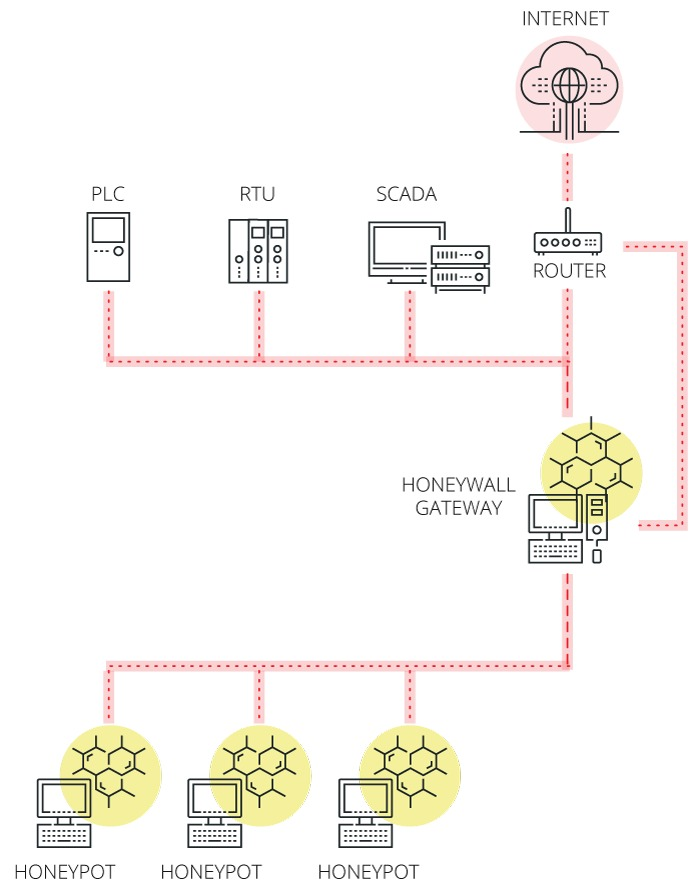
\includegraphics[scale=0.30]{figura_3.jpg}
\caption{Esquema de funcionamiento de los \textit{honeypots}}
\label{}
\end{figure}

\textbf{UML} permite ejecutar servicios de red y permanecer totalmente apartado del sistema Linux que soporta dicho sistema de virtualización, de modo que al ejecutar servicios de red en diferentes procesos \textbf{UML} de una misma máquina, estos permanecen aislados unos de otros, de forma que no pueden comprometer mutuamente la estabilidad o seguridad de los demás.
\\

\textit{Honeypot}, en español "tarro de miel", es una herramienta que se usa 
casi exclusivamente en el campo de la seguridad informática. Su función se 
basa en atraer y analizar ataques realizados por \textit{bots} o 
\textit{hackers}, para ver sus pautas de ataque, generar diccionarios para 
recopilar palabras que usan en ataques, conocer al enemigo y su perfil. 
También es posible utilizar dichos \textit{honeypots} para ralentizar el 
ataque (\textit{sticky honeypots}) y proteger así el resto del sistema. De 
esta forma, se tienen \textit{honeypots} de baja interacción, usados 
fundamentalmente como medida de seguridad, y \textit{honeypots} de alta 
interacción, capaces de reunir mucha más información y con fines como la 
investigación. De este modo, \textbf{UML} puede crear honeypots para simular 
redes locales de múltiples equipos, IPs falsas, directorios inventados... sin 
afectar al equipo.
\\

La virtualización también es importante para los desarrolladores. El núcleo 
de Linux ocupa un solo espacio de direcciones, lo que significa que un fallo 
en el núcleo o en cualquier \textit{driver} provoca la caída del sistema 
operativo completo. \textbf{UML} supone que puedes ejecutar varios sistemas 
operativos, y si uno cae debido a un fallo, el hipervisor y el resto de 
sistemas operativos continuarán funcionando debido a que son creados como 
procesos de usuario. Puesto que los núcleos se ejecutan en el espacio del 
usuario, deben estar compilados para este uso. Esto puede hacer que depurar 
el núcleo sea una tarea más parecida a depurar aplicaciones en el espacio de 
usuario.
\\

"UML permite disponer y configurar infraestructuras de red con un coste 
asumible para un laboratorio, y, a diferencia de los simuladores, muestra un 
comportamiento real del sistema", afirma un artículo que presenta la 
metodología que sigue la Facultad de Informática de la Universidad de Murcia 
en la asignatura de Redes. Practicar conceptos tales como encaminamiento, 
movilidad de IP, balanceo de carga y altadisponibilidad es lo que permite la 
herramienta de virtualización de código abierto \textbf{UML}. "Actualmente, 
la tasa de aprobados de las practicas está alrededor del 100\% ya que los 
alumnos, gracias a que pueden comprobar el funcionamiento de las soluciones 
planteadas, sólo las presentan cuando están seguros de que gran parte de los 
requisitos que se le piden a la solución funcionan." "Además, permite al 
profesor plantear, de la misma forma, casos inesperados a los que el alumno 
debería ser capaz de enfrentarse teniendo en cuenta lo aprendido durante la 
realización de la práctica." "De la aplicación de la metodología hemos 
recibido muchos comentarios positivos a lo largo de estos años" cita, entre 
otras, dicho artículo.
\\

Al no ser necesario que las versiones de kernel \textit{host} e invitado 
coincidan,  podemos ejecutar cualquier versión de Linux sobre la abstracción 
que proporciona dicho método de virtualización, como un proceso más del 
sistema operativo que lo soporta. Además, de este modo, otorgando más o menos 
recursos a dicho sistema operativo invitado, podemos concluir si un 
determinado equipo soporta dicha versión, incluso si es óptimo o no 
actualizar el equipo, facilitando así esta tarea y optimizando el uso del 
sistema operativo sobre un determinado hardware.
\\

La mayoría de aplicaciones están relacionadas con la consolidación de 
servidores. Si puedes ahorrar virtualizar un número de sistemas 
infrautilizados en un solo servidor, ahorrarás energía, espacio, capacidad de 
refrigeración y administración, ya que existen menos servidores. "Un servidor 
virtual actúa como si fuera una máquina entera dedicada a ti, pero de forma 
virtual. Es decir, disfrutas de muchas de las características de los 
servidores dedicados, pero la máquina física está compartida entre varios 
usuarios" defiende la página web \url{cdmon.com}, una página web que oferta 
servidores privados basados en esta técnica de virtualización. Ésta afirma 
"por un precio ajustado contarás con tecnología de última generación y la 
administración íntegra por parte de nuestros técnicos". Entre otras ventajas, 
destaca una nube 100\% privada, al no compartir ni la IP ni el sistema 
operativo con otros sitios web, posibilidad de ampliar tanto recursos como 
bases de datos como el número de \textit{hostings} soportados, recursos 
dedicados al tener una RAM dedicada, y; sobre todo, destaca su 
calidad/precio. Desde una perspectiva de negocio, hay muchas razones para
utilizar virtualización.

\section{Conclusiones}

En primer lugar, podríamos decir que \textit{user mode linux} (\textbf{UML}) 
es una herramienta de virtualización muy accesible, puesto que se encuentra 
disponible directamente para su uso en los sistemas GNU/Linux, por lo que en
caso de necesitar temporalmente un entorno virtual y no tener ninguna
preferencia sobre el software necesario para conseguirlo, puede ser la mejor
opción. Sin embargo, el hecho de no tener una interfaz gráfica integrada
dentro de la herramienta puede repeler a usuarios casuales o sin formación
informática. 
\\

En segundo lugar, el hecho de que \textbf{UML} aísle la máquina virtual del
resto del sistema proporciona mucha seguridad a la hora de trabajar. Que el
sistema real no se vea afectado por errores en el sistema virtual proporciona
una enorme cantidad de ventajas, puesto que podemos tomar "riesgos" al 
trabajar en ese entorno virtual sin ningún temor. Esto puede resultar muy
útil en el campo de la enseñanza, puesto que es muy usual cometer errores
en el proceso de aprendizaje, y en el caso de administración de sistemas esos
errores pueden ser fatales. Mediante esta herramienta ese problema es
solventado.
\\

Aunque pudiera parecer que esta herramienta de visualización no tendría
multitud de aplicaciones; no por sus prestaciones, sino por la existencia de
otras más conocidas, la realidad es la contraria. \textbf{UML} tiene multitud
de aplicaciones el campo de la ciberseguridad y en el campo de los servidores.
Es en estos campos donde las ventajas y características que posee sobre el
resto de software de virtualización se pueden aprovechar mejor. 
\\

Esto se ve de forma más clara en el campo de los servidores, puesto que 
gracias a la virtualización y, específicamente, a \textbf{UML}, podemos 
disponer de multitud de "servidores virtuales" sobre un mismo servidor 
físico, con lo que puedes contratar uno de estos servidores por un precio 
menor al que normalmente tendrías que pagar para disponer de cierta cantidad 
de recursos. Aparte de los beneficios económicos que proporciona esta técnica 
en el uso de servidores, podríamos decir que, en cierta medida, el uso de 
virtualización ayuda a que exista un menor consumo energético y de materiales
en la construcción y mantenimiento de servidores a escala mundial. Esto puede
llegar a ser importante, puesto que el número de páginas web, servicios de
almacenamiento en la nube, etc. no para de aumentar, y probablemente no pare
en un futuro cercano.
\\

En resumen, \textbf{UML} es una poderosa herramienta de virtualización con
multitud de aplicaciones y que proporciona un "entorno seguro" en el que 
cualquier usuario, ya sea un desarrollador de software o simplemente una 
persona curiosa que quiere "trastear" con un sistema, puede trabajar sin temer
por su máquina.

\section{Bibliografía}

\begin{itemize}[font={\color{rojooscuro}\bfseries},noitemsep,align=left]
\sloppy
\item \url{https://elpuig.xeill.net/Members/vcarceler/articulos/virtual-linux}
\item \url{http://his.sourceforge.net/honeynet/papers/uml/}
\item \url{https://www.uv.es/sto/charlas/2010_CIM/hvl-cim-2010-slides.pdf}
\item \url{http://profesores.elo.utfsm.cl/~agv/elo330/2s04/projects/UML/intro.htm}
\item \url{https://www.uv.es/sto/charlas/2010_CIM/hvl-cim-2010.html/index.html#user-mode-linux-http-user-mode-linux-sourceforge-net}
\item \url{http://opensourceforu.com/2010/09/user-mode-linux-setup-and-debug/}
\item \url{https://web2.clarkson.edu/class/cs644/kernel/setup/uml/uml.html}
\item \url{https://wiki.gentoo.org/wiki/User-mode_Linux/Guide}
\item \url{http://profesores.elo.utfsm.cl/~agv/elo330/2s04/projects/UML/
resumen.htm}
\item \url{http://user-mode-linux.sourceforge.net/old/UserModeLinux-HOWTO-8.html#ss8.1}
\item \url{https://en.wikipedia.org/wiki/User-mode_Linux}
\item \url{https://es.wikipedia.org/wiki/Honeypot}
\item \url{https://elpuig.xeill.net/Members/vcarceler/articulos/virtual-linux}
\item \url{https://upcommons.upc.edu/bitstream/handle/2099/11773/a20.pdf}
\item \url{https://www.cdmon.com/es/servidores/virtual-up}
\item \url{http://www.mulix.org/lectures/user-mode-linux-lkdsg-oct-2003/user_mode_linux.pdf}
\end{itemize}

\end{document}